%%%%%%%%%%%%%%%%%%%%%%%%%%%%%%%%%%%%%%%%%%%%%%%%%%%%%%%%%%%%%%%%%%%%%%%%%%%
%
% Template for a LaTex article in English.
%
%%%%%%%%%%%%%%%%%%%%%%%%%%%%%%%%%%%%%%%%%%%%%%%%%%%%%%%%%%%%%%%%%%%%%%%%%%%

\documentclass[11pt,twocolumn]{article}

% AMS packages:
\usepackage[left=1.5cm,top=1.5cm,right=1.5cm,bottom=2.5cm]{geometry} 
\usepackage{amsmath, amsthm, amsfonts}
\usepackage[utf8]{inputenc}
\usepackage{caption}
\usepackage{subcaption}
\usepackage{float}
\usepackage[position=top]{subfig}
\usepackage{paralist}
\usepackage{setspace}
\usepackage{graphicx}
\usepackage{multicol}
\usepackage{blindtext}
\usepackage{array,url,kantlipsum}
\usepackage{float}

% \Mark is probably provided by spconf, that I don't have
\newcommand{\Mark}[1]{\textsuperscript{#1}}

\begin{document}
\twocolumn[{%
 \centering
 \LARGE Compressible effect on particle acceleration in MHD turbulence \\[1.5em]
% \large First Author\Mark{1},
%        Second Author\Mark{2},
%        Third Author\Mark{1},
%        Fourth Author\Mark{2}
%    and Fifth Author\Mark{3}\\[1em]
 
\vspace*{0.5cm}

\begin{abstract}
\begin{center}
\noindent \normalsize The compressibility effect of the magnetohydrodynamics fields  on charged particle 
energization is studied in the context of test particle simulation. This problem is relevant 
to solar wind and solar corona due to the compressible nature of those astrophysical 
scenarios. We obtain the turbulent electromagnetic field using direct numerical simulation 
of MHD equations in a strong background magnetic field using pseudospectral method.  
In order to explore the compressible effect over the particle dynamic we performed two 
different numerical experiments: the incompressible case and two weak compressible cases 
changing the sound Mach number: for $M=0.25$ and $M=0.1$. Analyzing  the behavior of protons and 
electrons in that turbulent field which is well known to form aligned current sheets in the 
direction of the guide magnetic field,  we show that compressibility enhance the efficiency 
of proton acceleration and that energization is due to perpendicular electric field 
generated between currents sheets. On the other hand, electrons remains magnetized and showing 
an adiabatic behavior, and not effect of compressibility is observed.

\end{center}
\end{abstract}
\normalsize
}]
%\date{\vspace{-10px}}
%\maketitle
%\begin{multicols}{2}
\section*{Introduction}
Turbulence is ubiquitous phenomenon in many of astrophysical environments in which a wide  variety of temporal and spatial scales are involved, this is the case of solar wind and intellestar medium where the energy is transported from large scale to smaller scale up to kinetic scale where the energy is dissipated and damped. Turbulence is the results of no linear interaction between fluctuations of the velocity and magnetic fields, which leads to a spatial intermittency that is associated with coherent structures where the dissipation is concentrated in strong gradient regions,  that impacts on the heating, transport and particle acceleration in plasma (Mathheus et al. 2015).

The efficiency of MHD turbulence to accelerate charge particles and its importance in space physics has been reported by different authors [], but the great variety of scales involved in turbulence makes this problem a challenge which should include analytical and numerical approaches. On long  timescale (large eddy turnover times) the stochastic acceleration is governed and momentum diffusion is the main acceleration mechanism which has been applied for cosmic-ray energization mainly addressed by quasi-linear theory (QLT)[]. In the diffusion studies is commonly seen that MHD turbulence is represented as a random collection of wave, and that representation lacks of coherent structures that has an important role at particle scale.

For instance at proton inertial range which is the typical spatial scale where the dissipative effects become important is in the order of particle gyroradius and the coherent structures plays an important roll on particle acceleration. Dmitruk et al. 2004  using test particle simulation into frozen electromagnetic field obtained from direct numerical simulation (DNS) of MHD equations shows that particle energization at dissipation scale is due to current sheets and the acceleration mechanism depends on the particle gyroradii. 

Using a more sophisticated model but still Frozen turbulent electromagnetic field, Dalena et al 2012. shows the same results, electrons initially moving with Alfv\'en velocity and with a huge inertia experience parallel acceleration process by almost parallel electric field. On the other hand, protons are accelerated by a two stages process: initially are parallel accelerated and gaining substantial energy in a short time. Then, the current-sheet thickness is comparable with proton gyroradii and it encounter the edge of the current sheets and is accelerated perpendicularly.  


The compressible MHD turbulence effect on particle energization has been reported in the very large scale turbulence problems in diffusion studies. In Cho and Lazarian 2006. They studied the fast and slow particle diffusion in a weak and strong compressible MHD turbulence  using QLT, in the context of transit time damping (TTD) or in the wave-particle interaction as it represent  They show an enhancement of particle acceleration in supersonic turbulence by non-resonant acceleration in fast diffusion case.  Also they discuss about the possible particle energization by incompressible MHD turbulence in non-resonant way during long mean free paths.

Similarly, there are many reports on test particle pitch angle scattering in magnetohydrodynamic turbulence, Lynn et al 2013 studied th efficiency of second order Fermi acceleration by weak compressible MHD turbulence, running simultaneously the test particle and MHD fields, imposing a scattering rate, they found that compressible turbulence is important agent to produce no-thermal particles.  In addition, there are others studies where test particles and fields are simultaneously resolved, In Weid et al 2015. and Teaca et al. 2014, two very close works concerning in the incompressible MHD model that both use, analyzing the effect of the correlation between magnetic and velocity fields on pitch-angle scattering and particle acceleration respectively, they found that imbalanced turbulence (nonzero cross-helicity in the system) enhance the particle acceleration and also the pitch angle scattering.

Further to study the diffusion problem, we are interested in compressible effect on particle acceleration by coherent structures in the dissipation range, for that reason this work in in the line of study of test particles in a frozen electromagnetic field, keeping in mind that both situation, the frozen and  the dynamic turbulent fields, could represent different physical scenarios and may be involved different acceleration mechanisms. We study the effect of compressibility of turbulent field  on proton and electrons acceleration, for that we analyze the behavior of particles for three different cases: the incompressible case, and two weak compressible cases changing the sound Mach number. 

The organization of this paper is as follows:  In section 2  we describe the model employed in our investigation, the equations and properties of turbulent MHD fields and the test particle model including the parameters that correlate particles and fields, in section 3 we show the features of proton and electron dynamic and in section 4, we discuses about the our finding.

\section*{Model}

The macroscopic description of plasma is given by three-dimensional compressible MHD: the density continuity equation, the equation of motion, magnetic field induction equation, and the equation of state (1-4) respectively, which involves the fluctuations  of velocity field $u$, magnetic field $b$ and density $\rho$. We assume a large-scale magnetic field $B_0$ in z-direction, so the total magnetic field in plasma is $B = B_0 + b$

\begin{equation}
 \frac{\partial \rho}{\partial t} + \nabla \cdot (\textbf{u}\rho) = 0
\end{equation}

\begin{equation}
 \frac{\partial \textbf{u}}{\partial t} + \textbf{u} \cdot \nabla \textbf{u} = - \frac{\nabla p}{\rho} + \frac{\textbf{j} \times \textbf{B}}{4\pi\rho} 
 + \nu \left( \nabla^2 \textbf{u} +    \frac{\nabla \nabla \cdot \textbf{u} }{3} \right)
\end{equation}

\begin{equation}
\frac{\partial \textbf{B}}{\partial t} = \nabla \times (\textbf{u} \times \textbf{B}) + \eta \nabla^2 \textbf{B}
\end{equation}

\begin{equation}
 \frac{p}{\rho^{\gamma}} = cte
\end{equation}


Where $p$ the pressure, $\nu$ the viscosity, $\eta$ the magnetic diffusivity and $J=\nabla \times \textbf{B} $ is the current density. We assume the pressure as polytropic ($\gamma=5/3$), and consider two weak compressible regimes with Mach number ($M= \sqrt{\gamma p/\rho}$) iqual to $M=0.25$ and $M=0,1$; Additionally, in order to get a ground reference to measure the compressible effect on particle acceleration we consider an incompressible regimen (\nabla \cdot \textbf{u} = 0).

The magnetic and velocity fields are expressed in Alfv\'en speed units, a characteristic plasma velocity is given by the parallel wave propagation along magnetic field $v_A = B_0/\sqrt{4\pi\rho}$ and magentic field is given by the root mean square value \delta B = $\sqrt{\langle\textbf{B}^2\rangle}$. The density is expressed in units of $\rho_0$ a reference initial plasma density, the characteristic length scale $L$ of the order of the turbulence correlation lenght is used as lenght units, and the unit timescale is an eddy turnover time $t_0=L/v_A$.

The MHD equations are solved numerically using Fourier pseudospectral method with periodic boundary condition in a cube of size  $L_{box}=2\pi L$, the scheme ensure exact energy conservation for the continuous time spatially discrete equations. The discrete time integration is done with a second-order Runge-Kutta method and a  resolution of ($256^3$) Fourier modes is considered. The kinematic Reynolds number $R=v_AL/\nu$ and magnetic Reynolds numbers $R=v_AL/\eta$, which resume the strength of nonlinear terms in the MHD equations compared to the dissipation terms, we take $R=R_m= 1000$, which are limited here by available spatial resolution. We consider a decaying simulation from an initial state with the kinetic and magnetic field fluctuations populating an annulus in Fourier k-space that $ 3\leq k \leq4$, with a constant amplitude and random phase.

When the turbulence is fully-developed and a broad range of scale from outer scale $L$ to dissipation scale $l_d\approx 1/32$ contain energy, we take the MHD state for push the test particles using a frozen magentic,velocity and current density fields.

The behavior of a test particle in electromagnetic field obtained from MHD is described by nonrelativistic equation of motion:

\begin{equation}
  \frac{d\textbf{v}}{dt} = \alpha(\textbf{E} + \textbf{v} \times \textbf{B}), \ \ \ \  \frac{d\textbf{r}}{dt} = \textbf{v}
\end{equation}
 
The nondimensional electric field \textbf{E} is obtained for Ohm's law normalized with $E_0= v_A B_0/c$ as follows:

\begin{equation}
 \textbf{E} =  -\textbf{u}  \times \textbf{B} + \frac{\textbf{j}}{R_m} 
\end{equation}

Where adimensional parameter $\alpha$ relates particles and MHD field parameters:

\begin{equation}
\alpha=\frac{L}{\rho_{ii}}
\end{equation}
Where $\rho_{ii}$ is the proton inertial lenght given by $\rho_{ii}=m_pc/(e\sqrt{4\pi\rho_0})$. The $\alpha$ parameter represents the nominal particle gyroradii and measures the range of scales involved in the system, in general the fluctuations cover a broadband of the inertial range from slower timscale associated with $L$ at velocity $v_A$ of up to the faster timescale given by the inverse of particle gyroradii and then by ion inertial range ($\rho_{ii}$). One could expected a value $\alpha \gg 1$ specially for space physics and astrophysical plasmas where there are strong evidence of a wide range of scales. It is worthy notice that in MHD the range where the dissipation effects become noticeable is of the order of proton inertial range and for real value of $\alpha$ parameter represent a huge computational challenge due to numerical limitations. In order to taking into account the full range of scale of the system using three dimensional MHD simulation, we define the dissipation length of the system $l_d=1/32$ as was named above, which is the thickness of the currents sheets and it let us to capture the effect of coherent structures on particle acceleration.

Once steady-state turbulence has been achieved, 10000 test particles are randomly distributed on the computational box and the equation of motion of particles interacting with electromagnetic field are solved using the same second-order Runge-Kutta method, furthermore we use linear interpolation for field values on each particle position.


In addition, the particles are initialized in rest but in a pretty short time, the particles acquire a Gaussian distribution function with a rms value of the order of Alfven velocity, this phenomenon was discussed in Dalena et al. 2012 and it has an important consequences in parallel and perpendicular acceleration for both proton and electrons. Despite, it is well known that the particle gyroradius determine the acceleration process and our aim in this paper is to explore the compresion effect on acceleration of large and small particle gyroradii, in the next section we performed three diferent cases of strong magnetized MHD with $B_0=10$ for two compressible fields with the Mach number M=0.25 and M=0.1 respectively, and the incompressible cases. We present the behavior of one proton case with a nominal gyroradii $\alpha= 32$ which correspond with the same dissipation scale in this problem and two different small giroradii: real mass electron m_e=m_p/1836 ($\alpha=-58752$) and a fictitious electron with mass 66 times the mass of electron with corresponding $\alpha=-2112$ parameter.

\section*{Results}

A sketch of three-dimensional view of the z-component current density on the simulation box at $t=2t_0$ for incompressible and compressible with $M=0.25$ is shown in the Figure 1. It is observed the current sheets aligned in the direction of the magnetic field guide field, also it could be seen that in both cases the structures are similar but more corrugated in the compressible case and smoother in the incompressible case. Latter is because we used the same initial condition for all the simulation suited for this paper. the coherent structures like this is presented by the natural tendency of MHD equation and the neighborhood of sheets is governed others opposed sign current sheets leading to a many reconection zones that is the well known be the mechanism behind the acceleration of charged particles.

Figure 2 shows the total spectrum of kinetic (top) and magentic field (bottom)for the compressible $M=0.1$, $M=0.25$ and incompressible fields respectively. At inertial range there is almost no differences between compressible and incompressible energy spectrum for both magnetic and velocity fields. On the contrary, the energy contained at dissipation range changes for $k\gg32$, containing greater energy as mach number increases at this scales, this feature is more evident in kinetic energy than in magnetic field. It is remarkable that protons are mostly interacting with structures with that size and it could be an important effect on proton acceleration.

\begin{figure}[h!]
\begin{center}
{\includegraphics[width = 0.45\textwidth]{incompressible_256.eps}}\\
{\includegraphics[width = 0.45\textwidth]{compressible_256.eps}}
\caption{Three dimensional view of the parallel current density $J_z(x,v,z)$. (Left) Incompressible and 
(Right) Compressible field with Mach number $M=0.25$ case at $t/t_0 =2$.}
\end{center}
\end{figure}


\begin{figure}[h!]
\begin{center}
{\includegraphics[width = 3.5in]{spectrum_k.eps}}\\
{\includegraphics[width = 3.5in]{spectrum_m.eps}}
\caption{(Left). Total kinetic energy spectrum for compressible field with Mach number $M=0.25$ (solid line), $M=0.1$ (dashed line) and incompressible case (dash-dot line). (Right) Total Magnetic energy spectrum for the three cases named before using the same line type.}
\end{center}
\label{mean square velocity}
\end{figure}

The Figure 3 shows the time evolution of the perpendicular $\sqrt{v_x^2+v_y^2}$ rms velocity of protons (top) and z-component of velocity for real mass electrons (bottom) for the compressible $M=0.25$, $M=0.1$ and incompressible cases. The typical acceleration process observed in previous studies, proton are accelerated perpendicularly with respect to the magnetic field guide, and electrons are parallel accelerated. It should be mentioned that we present a really short time simulation of electrons because there are limitation in the choose of time step and huge computational resources is needed to represent a physical fast gyroradius of real mass electrons. The time reached in this electron simulation represents almost 3000 electron gyroperiods which is enough to observe the typical behavior of small particle gyroradius.

Moreover, compressible effect on particle acceleration is clearly observed, on the one hand, protons are highly accelerated as compressibility of the field increases, achieving almost three time higher velocity for twice Mach number in compressible field. Besides, the acceleration of protons in the incompressible case is less efficiently than the compressible one, but it is also observed that protons are accelerated but lower than in the compressible case.



\begin{figure}[h!]
\begin{center}
{\includegraphics[width = 3.5in]{Fig1.eps}}\\
{\includegraphics[width = 3.5in]{Fig2.eps}}
\caption{Particle mean square velocity as function of time in a static MHD turbulence: (Left) Ion 
perpendicular velocity $v_\perp = \sqrt{v_x^2 + v_y^2}$ for two different Mach number cases, 
$M=0.25$ (solid line), $M=0.1$ (dashed line) and incompressible case (dash-dot line). (Right) 
Electron parallel velocity for $M=0.25$, $M=0.1$ and incompressible field with the same line type.}
\end{center}
\label{mean square velocity}
\end{figure}

On the other hand, there is not evidence that compression of the MHD fields enhance the electron acceleration, in spite of the short time of that simulation, electrons gain the same energy at the end of each simulation.

\begin{figure}
\begin{center}
{\includegraphics[width = 3.5in]{elec_real_mu.eps}}
{\includegraphics[width = 3.5in]{elec_fic_mu.eps}}
\caption{Mean square magnetic moment $\mu = v_{\perp}^2/2B$ as function of time for two different small 
gyroradii particles: (Left) real electron mass $m_e = m_p/1836$ and (Right) fictitious electron mass 
$m_e_f = 66 m_e$ with the same line type used before for the different field cases.}
\end{center}
\label{mean square velocity}
\end{figure}
 
In order to deeply understand the behaviour of electrons in that turbulent structure, In Figure 4 we show the mean square value of magnetic moment of electrons for two different small particle gyroradius representing by real mass electron and fictitious mass electrones named above at the end of last section.

The magnetic momentun $\mu=W_\perp/2B$, where $W_\perp$ is the perpendicular energy of a particle, is one of the adiabatic invariance in the charged particles dynamic in a magnetic fields. it has a enormus consecuences in the dynamic of particles and determine how magnetized is particle, at the same time, how much trapped is a particle in a field line.

It is observed that both electrons cases shows a similar behavior,they remain magnetized during time evolution and it corresponds to a magentized behavior of small gyroradii particles, which at the same tie tell us that particle remain in the field line and gain parallel energy during the forward and back travel around field line between mirror points.

\begin{figure*}[h!]
\begin{center}
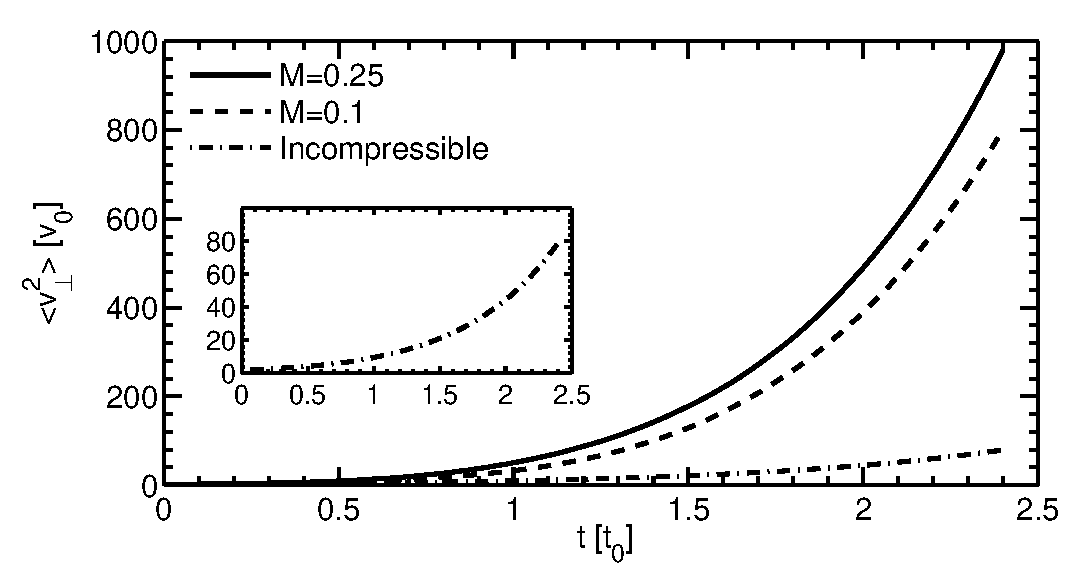
\includegraphics[width = 2.3in]{Fig3_a.eps}}
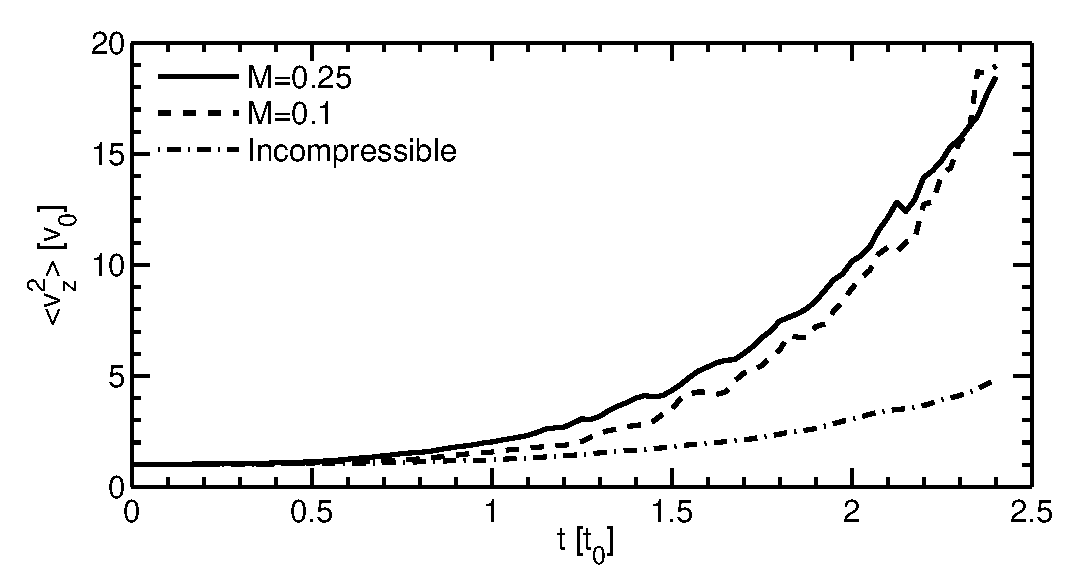
\includegraphics[width = 2.3in]{Fig3_b.eps}}
\includegraphics[width = 2.3in]{Fig3_c.eps}}
\caption{(a) Parallel current density, (b) three components of the electric field and (c) velocity 
components as function of time for the most energetic particle in each case: (Left) incompressible field,
(Middle) compressible $M=0.1$, and (Right) compressible $M=0.25$.}
\end{center}
\label{mean square velocity}
\end{figure*}
\twocolumn

sldkfsjdfjsdjfkljsdkjfklsdjfsdjfsjdfjsdjflsdjlfjsldjflksdjflsjfjsdjfslk


\begin{figure}[h!]
\begin{center}
{\includegraphics[width = 3.5in]{Fig4_1.eps}}
{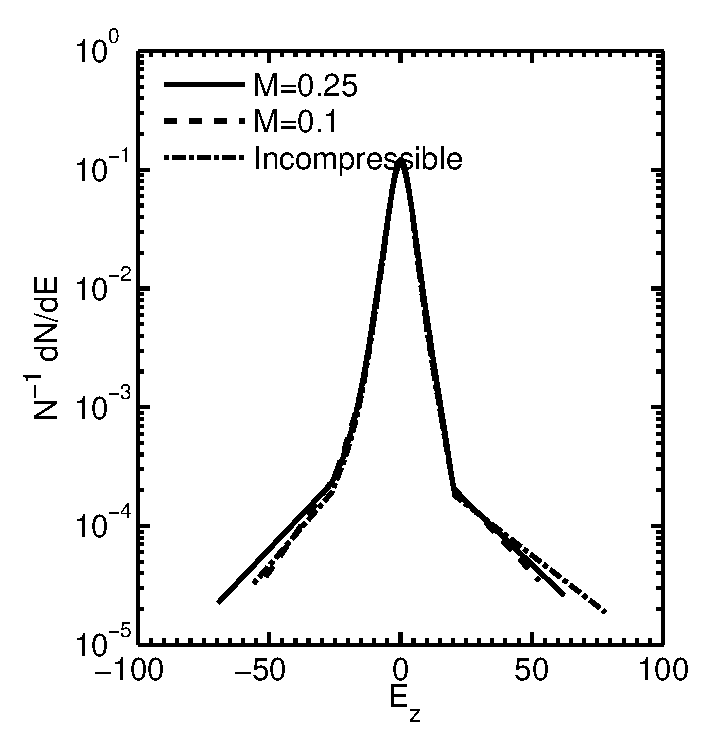
\includegraphics[width = 3.5in]{Fig4_2.eps}}
\caption{Probability density function of electric field in the simulation box. (Left) one of the 
component of perpendicular direction for $M=0.25$ (solid line), $M=0.1$ (dashed line) and 
incompressible field (dash-dot line). (Right) parallel component of electric field for the compressible 
and incompressible cases using the same line type.}
\end{center}
\label{mean square velocity}
\end{figure}



\clearpage                                                                                                                                                                                                                                                                                                                                                                                                                                                                                                                                                                                                                                                                                                                                                                                                                                                                                                                                                                                                                                                      
                                                                                                                                                                                                                                                                                                                                                                                                                                                                                                                                                                                                                                                                                                                                                                                                                                                                                                                                                                                                                                                                
                            

%\section*{Dynamic MHD turbulence}

%\begin{figure}[h!]
%\begin{center}
%{\includegraphics[width = 3.2in]{Fig5.eps}}
%{\includegraphics[width = 3.2in]{Fig5_2.eps}}
%\caption{Particle mean square velocity as function of time in a dynamic MHD turbulence: (Left) Ion 
%perpendicular velocity $v_\perp = \sqrt{v_x^2 + v_y^2}$ for two different Mach number cases, 
%$M=0.25$ (solid line), $M=0.1$ (dashed line) and incompressible case (dash-dot line). (Right) 
%Electron parallel velocity for $M=0.25$, $M=0.1$ and incompressible field with the same line type.}
%\end{center}
%\label{field}
%\end{figure}


%\begin{figure}[h!]
%\begin{center}
%\includegraphics[width = 2.3in]{Fig6_1.eps}}
%\includegraphics[width = 2.3in]{Fig6_2.eps}}
%\includegraphics[width = 2.3in]{Fig6_3.eps}}
%\caption{(a) Parallel current density, (b) three components of the electric field and (c) velocity 
%components as function of time for the most energetic particle in each case: (Left) incompressible field,
%(Middle) compressible $M=0.1$, and (Right) compressible $M=0.25$.}
%\end{center}
%\label{mean square velocity}
%\end{figure}
%\vspace{-0.5cm}

%\begin{figure}[h!]
%\begin{center}
%{\includegraphics[scale=0.5]{elec_real_mu_dyn.eps}}
%{\includegraphics[scale=0.5]{elec_fic_mu_dyn.eps}}
%\caption{Mean square magnetic moment $\mu = v_{\perp}^2/2B$ as function of time for two different small 
%gyroradii particles: (Left) real electron mass $m_e = m_p/1836$ and (Right) fictitious electron mass 
%$m_e_f = 66 m_e$ with the same line type used before for the different field cases.}
%\end{center}
%\label{mean square velocity}
%\end{figure}

%\section*{Particle energization differences between Static and Dynamic MHD turbulence}


%\begin{figure}[h!]
%\begin{center}
%{\includegraphics[width = 2in]{ion_dyn_stat_p.eps}}
%{\includegraphics[width = 2in]{ion_dyn_stat_z.eps}}
%\caption{Comparison of the probability density function of ion velocity for static (solid line) and 
%dynamic (dashed line) cases. (Left) Perpendicular velocity for compressible $M=0.25$ field at 
%$t/t_0 = 2.5$. (Right) Parallel ion velocity for the same cases at the same time.}
%\end{center}
%\label{mean square velocity}
%\end{figure}
%\vspace*{-0.5cm}
%\begin{figure}[h!]
%\begin{center}
%{\includegraphics[width = 2in]{elec_dis_dyn_stat_p.eps}}
%{\includegraphics[width = 2in]{elec_dis_dyn_stat_z.eps}}
%\caption{Comparison of the probability density function of real mass electron velocity for static (solid line) and 
%dynamic (dashed line) cases. (Left) Perpendicular velocity for compressible $M=0.25$ field at 
%$t/t_0 = 4.5x10^{-3}$. (Right) Parallel ion velocity for the same cases at the same time.}
%\end{center}
%\label{mean square velocity}
%\end{figure}





\end{document}  
